\section{Сложные случаи из практики}

\subsection{Пример картинки}

Рандомный граф (рис.~\ref{pic:graph}). 

Для насильной привязки к месту использовать опцию [H].

\begin{figure}[ht]
	\centering
	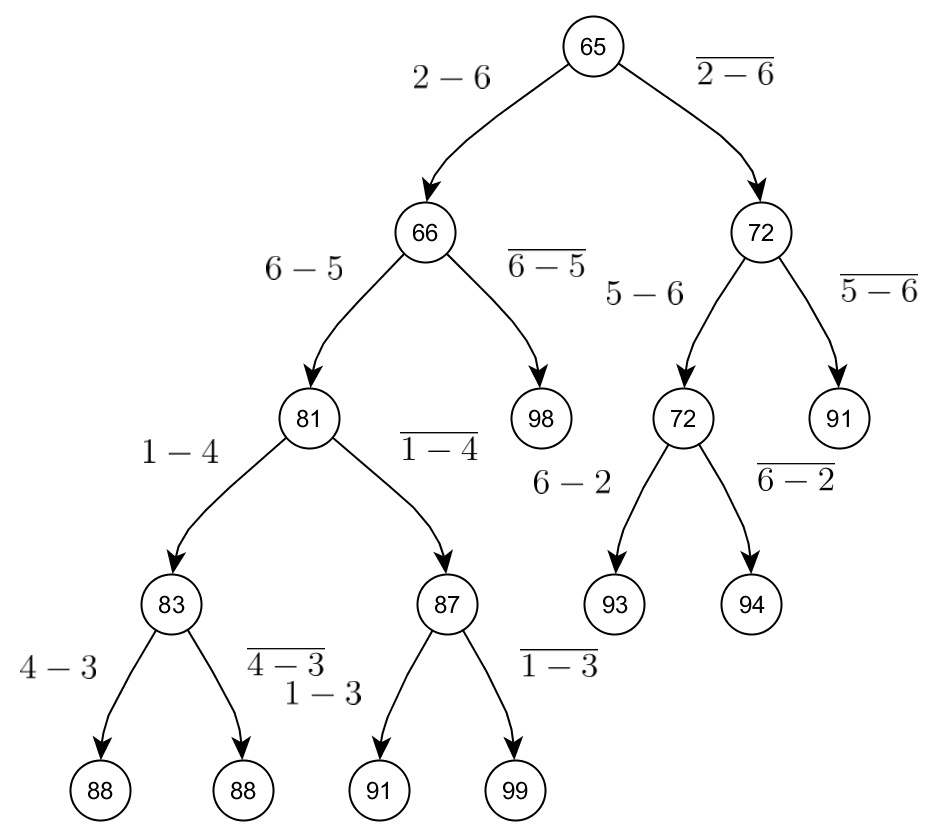
\includegraphics[width=0.6\textwidth]{full}
	\caption{Граф}
	\label{pic:graph}
\end{figure}

\subsection{Листинг с помощью listings}

Ад на земле.

\lstset{ %
language=VHDL,					% выбор языка для подсветки (здесь это С)
basicstyle=\small\sffamily,		% размер и начертание шрифта для подсветки кода
numbers=left,					% где поставить нумерацию строк (слева\справа)
numberstyle=\tiny,				% размер шрифта для номеров строк
stepnumber=2,					% размер шага между двумя номерами строк
numbersep=5pt,					% как далеко отстоят номера строк от подсвечиваемого кода
backgroundcolor=\color{white},	% цвет фона подсветки - используем \usepackage{color}
showspaces=false,				% показывать или нет пробелы специальными отступами
showstringspaces=false,			% показывать или нет пробелы в строках
showtabs=false,					% показывать или нет табуляцию в строках
frame=false,					% рисовать рамку вокруг кода
tabsize=2,						% размер табуляции по умолчанию равен 2 пробелам
captionpos=b,					% позиция заголовка вверху [t] или внизу [b] 
breaklines=true,				% автоматически переносить строки (да\нет)
breakatwhitespace=false,		% переносить строки только если есть пробел
escapeinside={\%*}{*)}			% если нужно добавить комментарии в коде
}

Описание схемы на языке VHDL приведено в листинге \ref{lst:VHDL}.
См. приложение~\ref{app:matlab} для ещё одного примера.

\begin{lstlisting}[label=lst:VHDL,caption=Описание схемы]
entity lab2 is
port(
SW0,SW1,SW2,SW3,SW4:in bit;
LED0,LED1,LED2:out bit;
LED3,LED4,LED5:out boolean);
end lab2;
architecture rtl of lab2 is
	signal TEMP:bit:='0';
begin
LED2<='0';
temp<=SW0 or SW1;
LED1<=TEMP and SW2;
LED0<=not TEMP;
LED3<=not(SW3>SW4);
LED4<=not(SW3=SW4);
LED5<=not(SW3<SW4);
end rtl;
\end{lstlisting}

\subsection{Картинки с подкартинками}

Данные о максимальной частоте и минимальных временных задержках представлены на рис. \ref{pic:base} (а так же рис.~\ref{pic:fmax} и рис.~\ref{pic:clk}).

\begin{figure}[h]
	\begin{subfigure}{.4\linewidth}\centering
		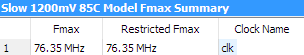
\includegraphics[width=1\textwidth]{fmax}
		\caption{Максимальная частота}
		\label{pic:fmax}
	\end{subfigure}
	\begin{subfigure}{.6\linewidth}\centering
		
\includegraphics[width=1\textwidth]{clk}
		\caption{Минимальные задержки}
		\label{pic:clk}
	\end{subfigure}
\caption{Описание без оптимизации}
\label{pic:base}
\end{figure}

\subsection{Длинная подпись}

Результат моделирования синтезированной схемы представлен на рис. \ref{pic:modeling}. 

\begin{figure}[ht]
\centering
\captionsetup{justification=centering} % Вот эта строка, в принципе можно внести в шаблон, но я поленился, плюс есть случай, когда её лучше не переопределять
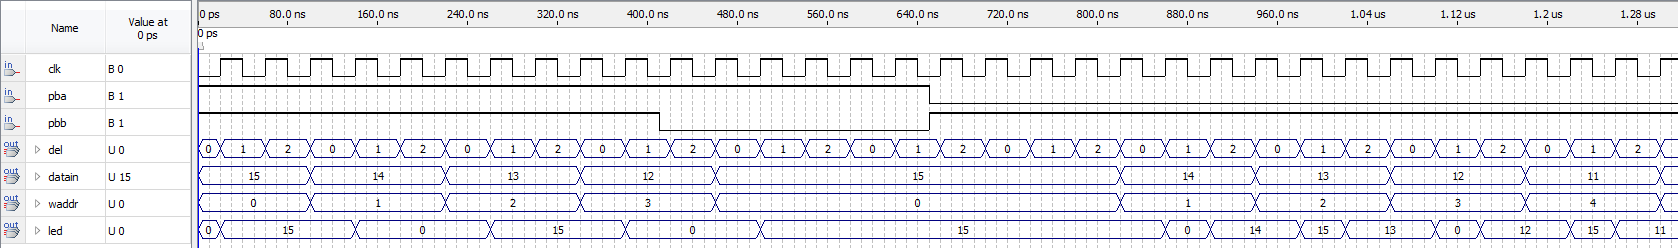
\includegraphics[width=1\textwidth]{modeling}
\caption{Результат моделирования схемы в редакторе диаграмм \\ (Коэффициент деления частоты = 3)}
\label{pic:modeling}
\end{figure}

А вот и пример такого случая (см. табл. \ref{tab:task}).

\begin{table}[H]
	\centering
	\captionsetup{justification=raggedleft}
	\caption{Результат моделирования схемы в редакторе диаграмм \\ (Коэффициент деления частоты = 3)}
	\begin{tabular}{|c|c|c|c|c|c|}
		\hline $\infty$& $27$ & $13$ & $7$ & $45$ & $35$ \\
		\hline $21$ & $\infty$ & $14$ & $20$ & $19$ & $12$ \\
		\hline $10$ & $14$ & $\infty$ & $6$ & $32$ & $25$ \\
		\hline $7$ & $18$ & $5$ & $\infty$ & $38$ & $28$ \\
		\hline $32$ & $16$ & $23$ & $27$ & $\infty$ & $23$ \\
		\hline $30$ & $10$ & $24$ & $28$ & $18$ & $\infty$ \\
		\hline		
	\end{tabular}
	\label{tab:task}
\end{table}

\subsection{Русские буквы в формулах}

Пока только такой вариант (\ref{eq:rus}).

\begin{equation}
	\sum_{\textup{Какая-то лажа}}^{\textit{Какой-то курсив}} \textbf{Какой-то жирнич}
	\label{eq:rus}
\end{equation}

\subsection{Отрицание-подчёркивание в мат. режиме}

Просто $\overline{\textup{над}}~\underline{\textup{под}}$

Ещё пример (в двух вариантах форматирования кода, на мой взгляд, оба отстойны):

\centerline{\large$y = \overline{\overline{\overline x_{3}x_{4}\overline{\overline{\overline x_{1}\overline x_{2}}\overline x_{5}}}~\overline{x_{2}\overline{\overline x_{1}\overline{x_{4}x_{5}}}}~\overline{x_{3}\overline{\overline{\overline x_{1}\overline x_{4}}\,\overline{\overline x_{2}\overline x_{5}}}}}$} \normalsize ~\\

\centerline{
	\large$y = \overline{
		\overline{
			\overline x_{3}x_{4}\overline{
				\overline{
					\overline x_{1}\overline x_{2}
				}
				\overline x_{5}
			}
		}
		~\overline{
			x_{2}\overline{
				\overline x_{1}\overline{
					x_{4}x_{5}
				}
			}
		}
		~\overline{
			x_{3}\overline{
				\overline{
					\overline x_{1}\overline x_{4}
				}
				\,\overline{
					\overline x_{2}\overline x_{5}
				}
			}
		}
	}
	$} \normalsize 

\subsection{No line here to end при использовании \textbackslash\textbackslash}

Способ в формуле выше, создать минимальное пространство с помощью \textasciitilde~перед \textbackslash\textbackslash, или использовать \string\vspace\{X pt\}.

\subsection{Таблица с картинкой}

Пример в табл.~\ref{tab:rs-map}.

\begin{table}[ht]
\centering
\begin{tabular}{|c|c|c|}
\hline Имя & Функциональный преобразователь & Логическое выражение выходов \\
\hline inst & \raisebox{-\totalheight}{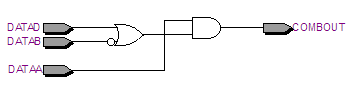
\includegraphics[width=0.45\textwidth]{rs-inst}} & \specialcell{\\ $\overline{(Q'+\overline{R})\cdot S}\rightarrow Q$} \\
\hline inst1 & \raisebox{-\totalheight}{
\includegraphics[width=0.45\textwidth]{rs-inst1}} &  \specialcell{\\$\overline{\overline{Q''} \cdot R}\rightarrow \overline{Q}$} \\ \hline
\end{tabular}
\caption{Логические выражения для выходов RS-триггера}
\label{tab:rs-map}
\end{table}

\subsection{Таблица с склееными и битыми ячейками}

Пример в табл.~\ref{tab:energy}.

\begin{table}[H]
\centering
\begin{tabular}{|c||*{4}{c|}}
\hline \multirow{2}*{\textnumero} & \multirow{2}*{Частота, МГц} & \multirow{2}*{Период, нс} & \multicolumn{2}{c|}{Энергопотребление, мВт}\\
\cline{4-2}\cline{5-2}  & & & Полное & Динамическое \\
\hline 1 & 1 & 1000 & 64.79 & 0.05\\
\hline 2 & 10 & 100 & 65.45 & 0.51\\
\hline 3 & 50 & 20 & 68.38 & 2.53\\
\hline 4 & 100 & 10 & 72.05 & 5.06\\
\hline 5 & 150 & 6.667 & 75.71 & 7.59\\
\hline 6 & 200 & 5 & 79.38 & 10.13\\
\hline 7 & 250 & 4 & 83.05 & 12.66 \\ \hline
\end{tabular}
\caption{Зависимость энергопотребления от частоты}
\label{tab:energy}
\end{table}

\subsection{Графики с pgfplots/tikZ}

Слишком потно, надо очень хорошо знать, что делаешь, иначе можно потратить день и не добиться результата. В документации 600 страниц, Карл!!!

\begin{figure}[h]
	\begin{subfigure}{.5\linewidth}\centering
		\begin{tikzpicture}
			\begin{axis}[
				grid = both,
				axis line style = very thick,
				axis x line=bottom,
				axis y line=left,
				xlabel = {$f$, МГц},
    			ylabel = {$W$, мВт},
    			minor tick num = 1]
			\addplot coordinates {
    			(1,0.05) (10,0.51) (50,2.53) (100,5.06) (150,7.59) (200,10.13) (250,12.66)
			};
			\end{axis}
		\end{tikzpicture}
		\caption{Динамическое}
		\label{gr:din}
	\end{subfigure}
	\begin{subfigure}{.5\linewidth}\centering
		\begin{tikzpicture}
			\begin{axis}[
				grid = both,
				axis line style = very thick,
				axis x line=bottom,
				axis y line=left,
				xlabel = {$f$, МГц},
		  		ylabel = {$W$, мВт},
    			minor tick num = 1]
			\addplot coordinates {
    			(1,64.79) (10,65.45) (50,68.38) (100,72.05) (150,75.71) (200,79.38) (250,83.05)
			};
			\end{axis}
		\end{tikzpicture}
		\caption{Полное}
		\label{gr:stat}
	\end{subfigure}
\caption{Зависимость энергопотребления от частоты}
\label{gr:energy}
\end{figure}

\subsection{Надписи на стрелках}

Использует пакет $mathtools$.

\begin{table}[h!t]
\centering
\begin{tabular}{|c|cc|c|}
\hline & $x_3$ & $x_2$ & $B$ \\
\hline $x_1$ & $-1$ & $-0.3$ & $10.2$ \\
 $x_4$ & $-1$ & $-0.7$ & $11.4$ \\
\hline $x_5$ & \textbf{2.5} & $-0.25$ & \textbf{-10.5} \\
\hline $f$ & \textbf{-1} & $-2.3$ & $10.2$ \\ \hline
\end{tabular}
$\xRightarrow[\text{делим на 2.5}]{\text{преобразуем и}}$
\begin{tabular}{|c|cc|c|}
\hline & $x_5$ & $x_2$ & $B$ \\
\hline $x_1$ & $-0.4$ & $-0.4$ & $6$\\
 $x_4$ & $-0.4$ & $-0.8$ & $7.2$ \\
 $x_3$ & $0.4$ & $0.1$ & $4.2$\\
\hline $f$ & $-0.4$ & $-2.4$ & $6$ \\ \hline
\end{tabular}
\end{table}

\subsection{Случай с матрицей, где проверялся знак}

Текущие матрицы $P=\begin{bmatrix}
0 & 1 \\ 1 & -1
\end{bmatrix}$, $C^B=\begin{bmatrix}
0 & 1
\end{bmatrix}$

Допустимость: $X^B=P^{-1}B=\begin{bmatrix}
11.4 \\ 10.2
\end{bmatrix}\begin{matrix}
>0 \\ >0
\end{matrix}$ -- \textbf{допустимый}

\subsection{Скобочка}

\begin{equation*}
\left\{\begin{aligned}
\max\left(x_1-2x_2\right), \\
x_1+0.3x_2\leq 10.2, \\
-x_1+0.4x_2\leq 1.2, \\
x_1\geq 0, \\
x_2\geq 0; \\
\end{aligned}\right. \Longleftrightarrow
\left\{\begin{aligned}
\max\left(x_1-2x_2\right), \\
x_1+0.3x_2+x_3=10.2, \\
-x_1+0.4x_2+x_4=1.2, \\
x_1\geq 0, \\
x_2\geq 0; \\
x_3\geq 0, \\
x_4\geq 0; \\
\end{aligned}\right.
\end{equation*}

\subsection{Сторона прижатия в выражениях}

Прижатие контролируется символом \&. \\

Условия Куна-Такера:
\begin{equation}
\left\{\begin{aligned}
&\nabla f(X^*)+\sum_{j=1}^{J} u_j \nabla g_j(X^*)=0,\\
&u_j g_j(X^*)=0,~ j=1..J,\\
&u_j \leq 0,~ j=1..J;\\
\end{aligned}\right.
\label{kung}
\end{equation}

Подставим в формулу \eqref{kung}:

\begin{equation*}
\left\{\begin{aligned}
-62x_1+4x_2+286+7u_1+10u_2-u_3=0,\\
-68x_2+4x_1+388+12u_1+8u_2-u_4=0,\\
u_1(7x_1+12x_2-84)=0,\\
u_2(10x_1+8x_2-80)=0,\\
u_3(-x_1)=0,\\
u_4(-x_2)=0,\\
u_1\leq 0,\\
u_2\leq 0,\\
u_3\leq 0,\\
u_4\leq 0;\\
\end{aligned}\right.
\end{equation*}

\subsection{Графы}

Безумно неудобно, не делать так. Лучше, быстрее и выгоднее заюзать yEd или что-нибудь в таком духе и вставить картинку. Есть способ делать удобнее с LuaTeX, но LuaTeX сам по себе ещё без релизной версии, ну его к чёрту. \\

Наибольший путь $1-2-4-5-6-7-8$ с весом $39$ представлен на рис. \ref{pic:graph_max}.

\begin{figure}[H]
	\centering
	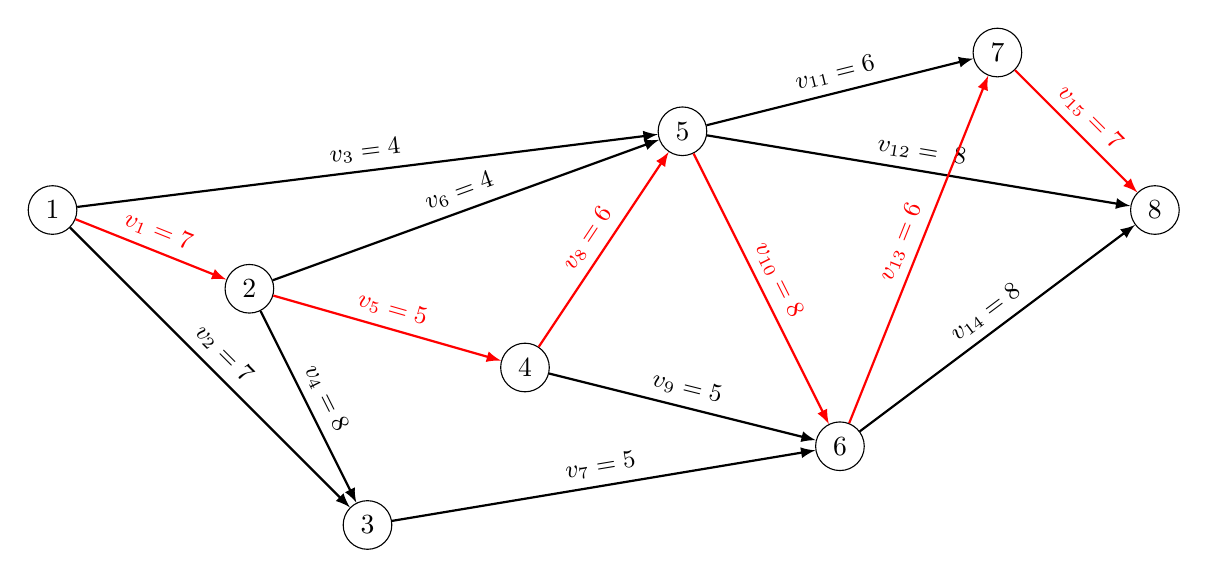
\begin{tikzpicture}[scale = 2]
		\node [circle,draw] (l1) at (0,2) {1};
		\node [circle,draw] (l2) at (1.25,1.5) {2};
		\node [circle,draw] (l3) at (2,0) {3};
		\node [circle,draw] (l4) at (3,1) {4};
		\node [circle,draw] (l5) at (4,2.5) {5};
		\node [circle,draw] (l6) at (5,0.5) {6};
		\node [circle,draw] (l7) at (6,3) {7};
		\node [circle,draw] (l8) at (7,2) {8};
		\path[->, thick, >=latex]
					(l1) edge[red] node[sloped, above]{\small $v_1=7$} (l2)
					(l1) edge node[sloped, above]{\small $v_2=7$} (l3)
					(l1) edge node[sloped, above]{\small $v_3=4$} (l5)
					(l2) edge node[sloped, above]{\small $v_6=4$} (l5)
					(l2) edge[red] node[sloped, above]{\small $v_5=5$} (l4)
					(l2) edge node[sloped, above]{\small $v_4=8$} (l3)
					(l3) edge node[sloped, above]{\small $v_7=5$} (l6)
					(l4) edge[red] node[sloped, above]{\small $v_8=6$} (l5)
					(l4) edge node[sloped, above]{\small $v_9=5$} (l6)
					(l5) edge[red] node[sloped, above]{\small $v_{10}=8$} (l6)
					(l5) edge node[sloped, above]{\small $v_{11}=6$} (l7)
					(l5) edge node[sloped, above]{\small $v_{12}=~8$} (l8)
					(l6) edge[red] node[sloped, above]{\small $v_{13}=6$} (l7)
					(l6) edge node[sloped, above]{\small $v_{14}=8$} (l8)
					(l7) edge[red] node[sloped, above]{\small $v_{15}=7$} (l8);
	\end{tikzpicture}
\caption{Наибольший путь}
\label{pic:graph_max}
\end{figure}

\subsection{ИИИЛИТНЫЕ зачёркивания}

Пример: \\

$\begin{aligned}
	&2-6, 6-5, 1-4, 4-3 \Rightarrow \xcancel{6-2}, \xcancel{5-6}, \xcancel{5-2}, \xcancel{4-1}, \xcancel{4-2}, \xcancel{3-4}, \xcancel{3-1} \\
	&G_{2-6;6-5;1-4}=G_{2-6;6-5;1-4;4-3}\cup G_{2-6;6-5;1-4;\overline{4-3}} \\
\end{aligned}$ \\

Нельзя использовать зачёркивания пакета $cancel$ с самого первого слова: \\

\mbox{}\bcancel{Ещё} \cancel{такие} \st{вот} \xcancel{иногда} $\cancelto{\textup{варианты}}{\textup{есть}}$.

\section{Создание списка литературы}

Для этого можно использовать \textit{BiBLaTeX+Biber}.\cite{modelcheck}

Создаёт и нумерует ссылки в порядке их упоминания.\cite{shosh} Стиль по ГОСТу (\textit{gost-numeric} в данном шаблоне) и его использование можно почитать в описании стиля.\cite{gost}

\newpage
\phantomsection
\addcontentsline{toc}{section}{Список литературы} 
\printbibliography

\begin{append}
	
	\section{Ещё один пример листинга} \label{app:matlab}

	\lstset{language=Matlab,
		inputencoding=cp1251,
		basicstyle=\small\sffamily, 
	    breaklines=true,
	    morekeywords={matlab2tikz},
	    keywordstyle=\color{blue},
	    morekeywords=[2]{1}, keywordstyle=[2]{\color{black}},
	    identifierstyle=\color{black},
	    stringstyle=\color{mylilas},
	    commentstyle=\color{mygreen},
	    showstringspaces=false,
	    numbers=left,
	    numberstyle={\tiny \color{black}},
	    numbersep=5pt,
	    emph=[1]{for,break},emphstyle=[1]\color{red},
	    frame=single,
	    stepnumber=5,
	}

	\definecolor{mygreen}{RGB}{28,172,0} % color values Red, Green, Blue
	\definecolor{mylilas}{RGB}{170,55,241}

	\lstinputlisting[firstline=1, lastline=91]{code/Main.m}

	\section{Ссылка вида ``<буква>'' $\wedge$\_$\wedge$}

	Поставленные требования к оформлению приложений выполнены, за исключением капитализации, так как она смотрелась неуместно.

	\subsection{Одна подсекция}

	Вот она!

	\subsection{Ещё одна подсекция}

	\Huge$\backslash O /$

\end{append}

